\section{Technical Considerations}

\subsection{Data Extraction}

In order to extract content from multiple web pages, a web crawler will need to be created using the Python programming language. The group plans on using Scrapy, a Python library which will handle the "`visiting"' of websites, when provided with a sufficient list of hosts. Scrapy crawls through each directory within the host (as defined by the site's \textsl{robots.txt} file). After visiting a URL, the content will be extracted and analysed using the information retrieval methods available in the Python Natural Language Toolkit (NLTK) library.

\begin{figure}
  \centering
  \begin{minipage}{7cm}
    \centering
    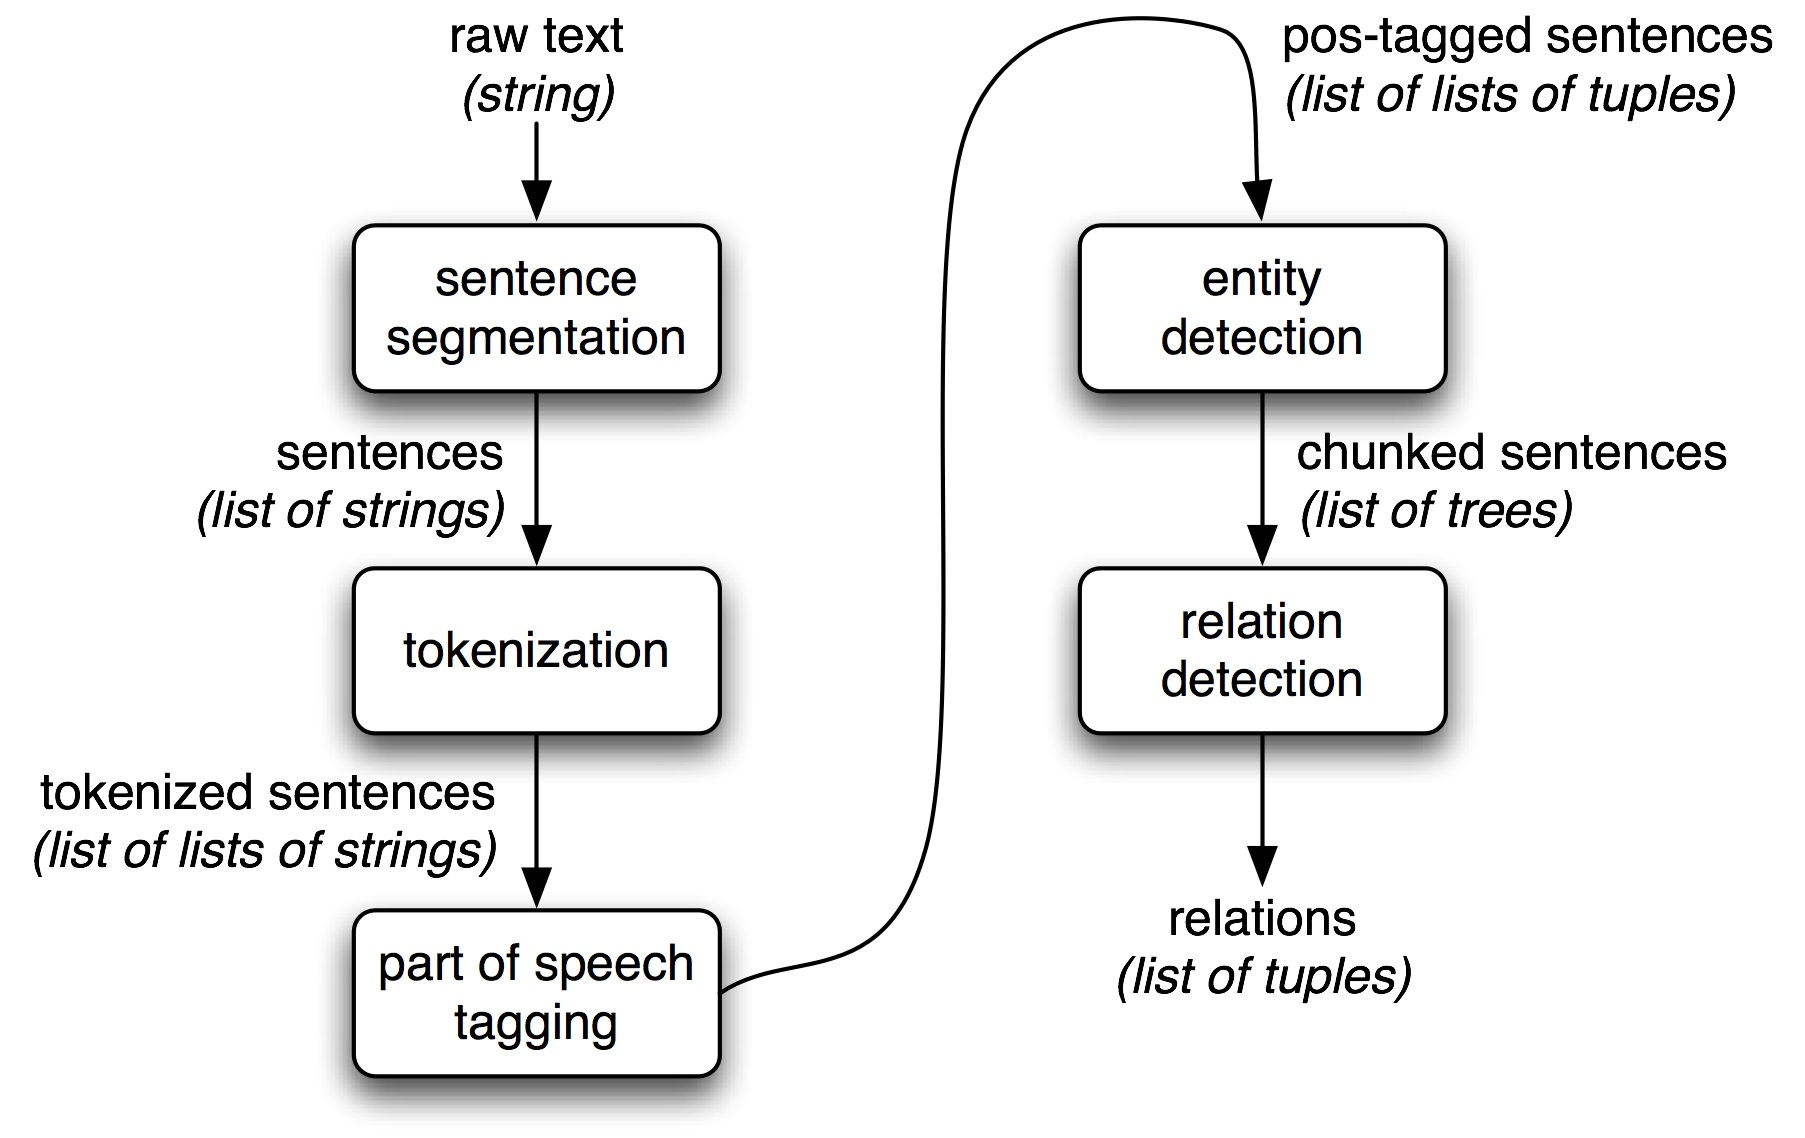
\includegraphics[width=7cm]{inc/ie-architecture.jpg}
    \caption{Python Natural Language Tookit Information Retrieval Flow Diagram}
    \label{fig:information_retrieval}
  \end{minipage}
\end{figure}

Many websites implement measures to prevent web crawlers from crawling due to the number of requests made as they utilise their server resources. Quite often, this results in the crawler being banned. However, the group can take the following measures to prevent this:

\begin{itemize}
  \item Disabling cookies may prevent getting banned, but only if it’s the method used by the website to detect crawlers
  \item Using Google cached pages instead of visiting the websites directly
  \item Using different IP addresses by rotating from a list when making a request to the same host
  \item Setting a delay between requests
\end{itemize}

\subsection{Sentiment Analysis}

Once the user's online content has been extracted, it will then placed into one of the following categories: negative, positive or neutral. This can be achieved by performing sentiment analysis on the content. However, the app's back-end has to be first be trained by supplying sufficient training data.

The language used for the sentiment analysis will be Python. Moreover, the group will also make use of the Natural Language Toolkit (NLTK) Python library.

\subsubsection{Data Collection \& Pre-Processing}

The first step is to collect existing positive, negative and neutral content and store them in an array.

\begin{figure}[h!]
  \centering
  \begin{minipage}{14cm}
    \centering
    \inputminted[fontsize=\footnotesize]{python}{inc/snippets/collection.py}
    \caption{Content Collection}
    \label{fig:sentiment_analysis_step1a}
  \end{minipage}
\end{figure}

These words are then collected into a single list of tuples, each of which containing two elements.

\begin{figure}[h!]
  \centering
  \begin{minipage}{14cm}
    \centering
    \inputminted[fontsize=\footnotesize]{python}{inc/snippets/collection_iteration.py}
    \caption{Content Pre-Processing}
    \label{fig:sentiment_analysis_step1b}
  \end{minipage}
\end{figure}

\subsubsection{Classifier Creation}

Once sufficient content has been attained, a list of each word extracted from all the content needs to be collected and then ordered based on frequency of occurrence. This can be done by initially collecting all words and associating a frequency of occurrence to each and then ordering the list based on the frequency value. 

\begin{figure}[h!]
  \centering
  \begin{minipage}{14cm}
    \centering
    \inputminted[fontsize=\footnotesize]{python}{inc/snippets/classifier.py}
    \caption{Word Frequency}
    \label{fig:sentiment_analysis_step2a}
  \end{minipage}
\end{figure}

To create the classifier, relevant features needs to be captured via a feature extractor.

\begin{figure}[h!]
  \centering
  \begin{minipage}{14cm}
    \centering
    \inputminted[fontsize=\footnotesize]{python}{inc/snippets/classifierB.py}
    \caption{Feature Extraction}
    \label{fig:sentiment_analysis_step2b}
  \end{minipage}
\end{figure}

A training set will then be created using the NLTK library. Furthermore, a classifier object can be instantiated.

\begin{figure}[h!]
  \centering
  \begin{minipage}{14cm}
    \centering
    \inputminted[fontsize=\footnotesize]{python}{inc/snippets/classifierC.py}
    \caption{Classifier Training}
    \label{fig:sentiment_analysis_step2b}
  \end{minipage}
\end{figure}

\subsubsection{Classifier Testing}

Now that the classifier has been created and trained, the sentiment analyser can be tested.

\begin{figure}[h!]
  \centering
  \begin{minipage}{14cm}
    \centering
    \inputminted[fontsize=\footnotesize]{python}{inc/snippets/classify.py}
    \caption{Classifier Testing}
    \label{fig:sentiment_analysis_step3}
  \end{minipage}
\end{figure}

\clearpage
\begin{landscape}

\section{System Architecture Diagram}

\begin{figure}
  \centering
  \begin{minipage}{180mm}
    \centering
    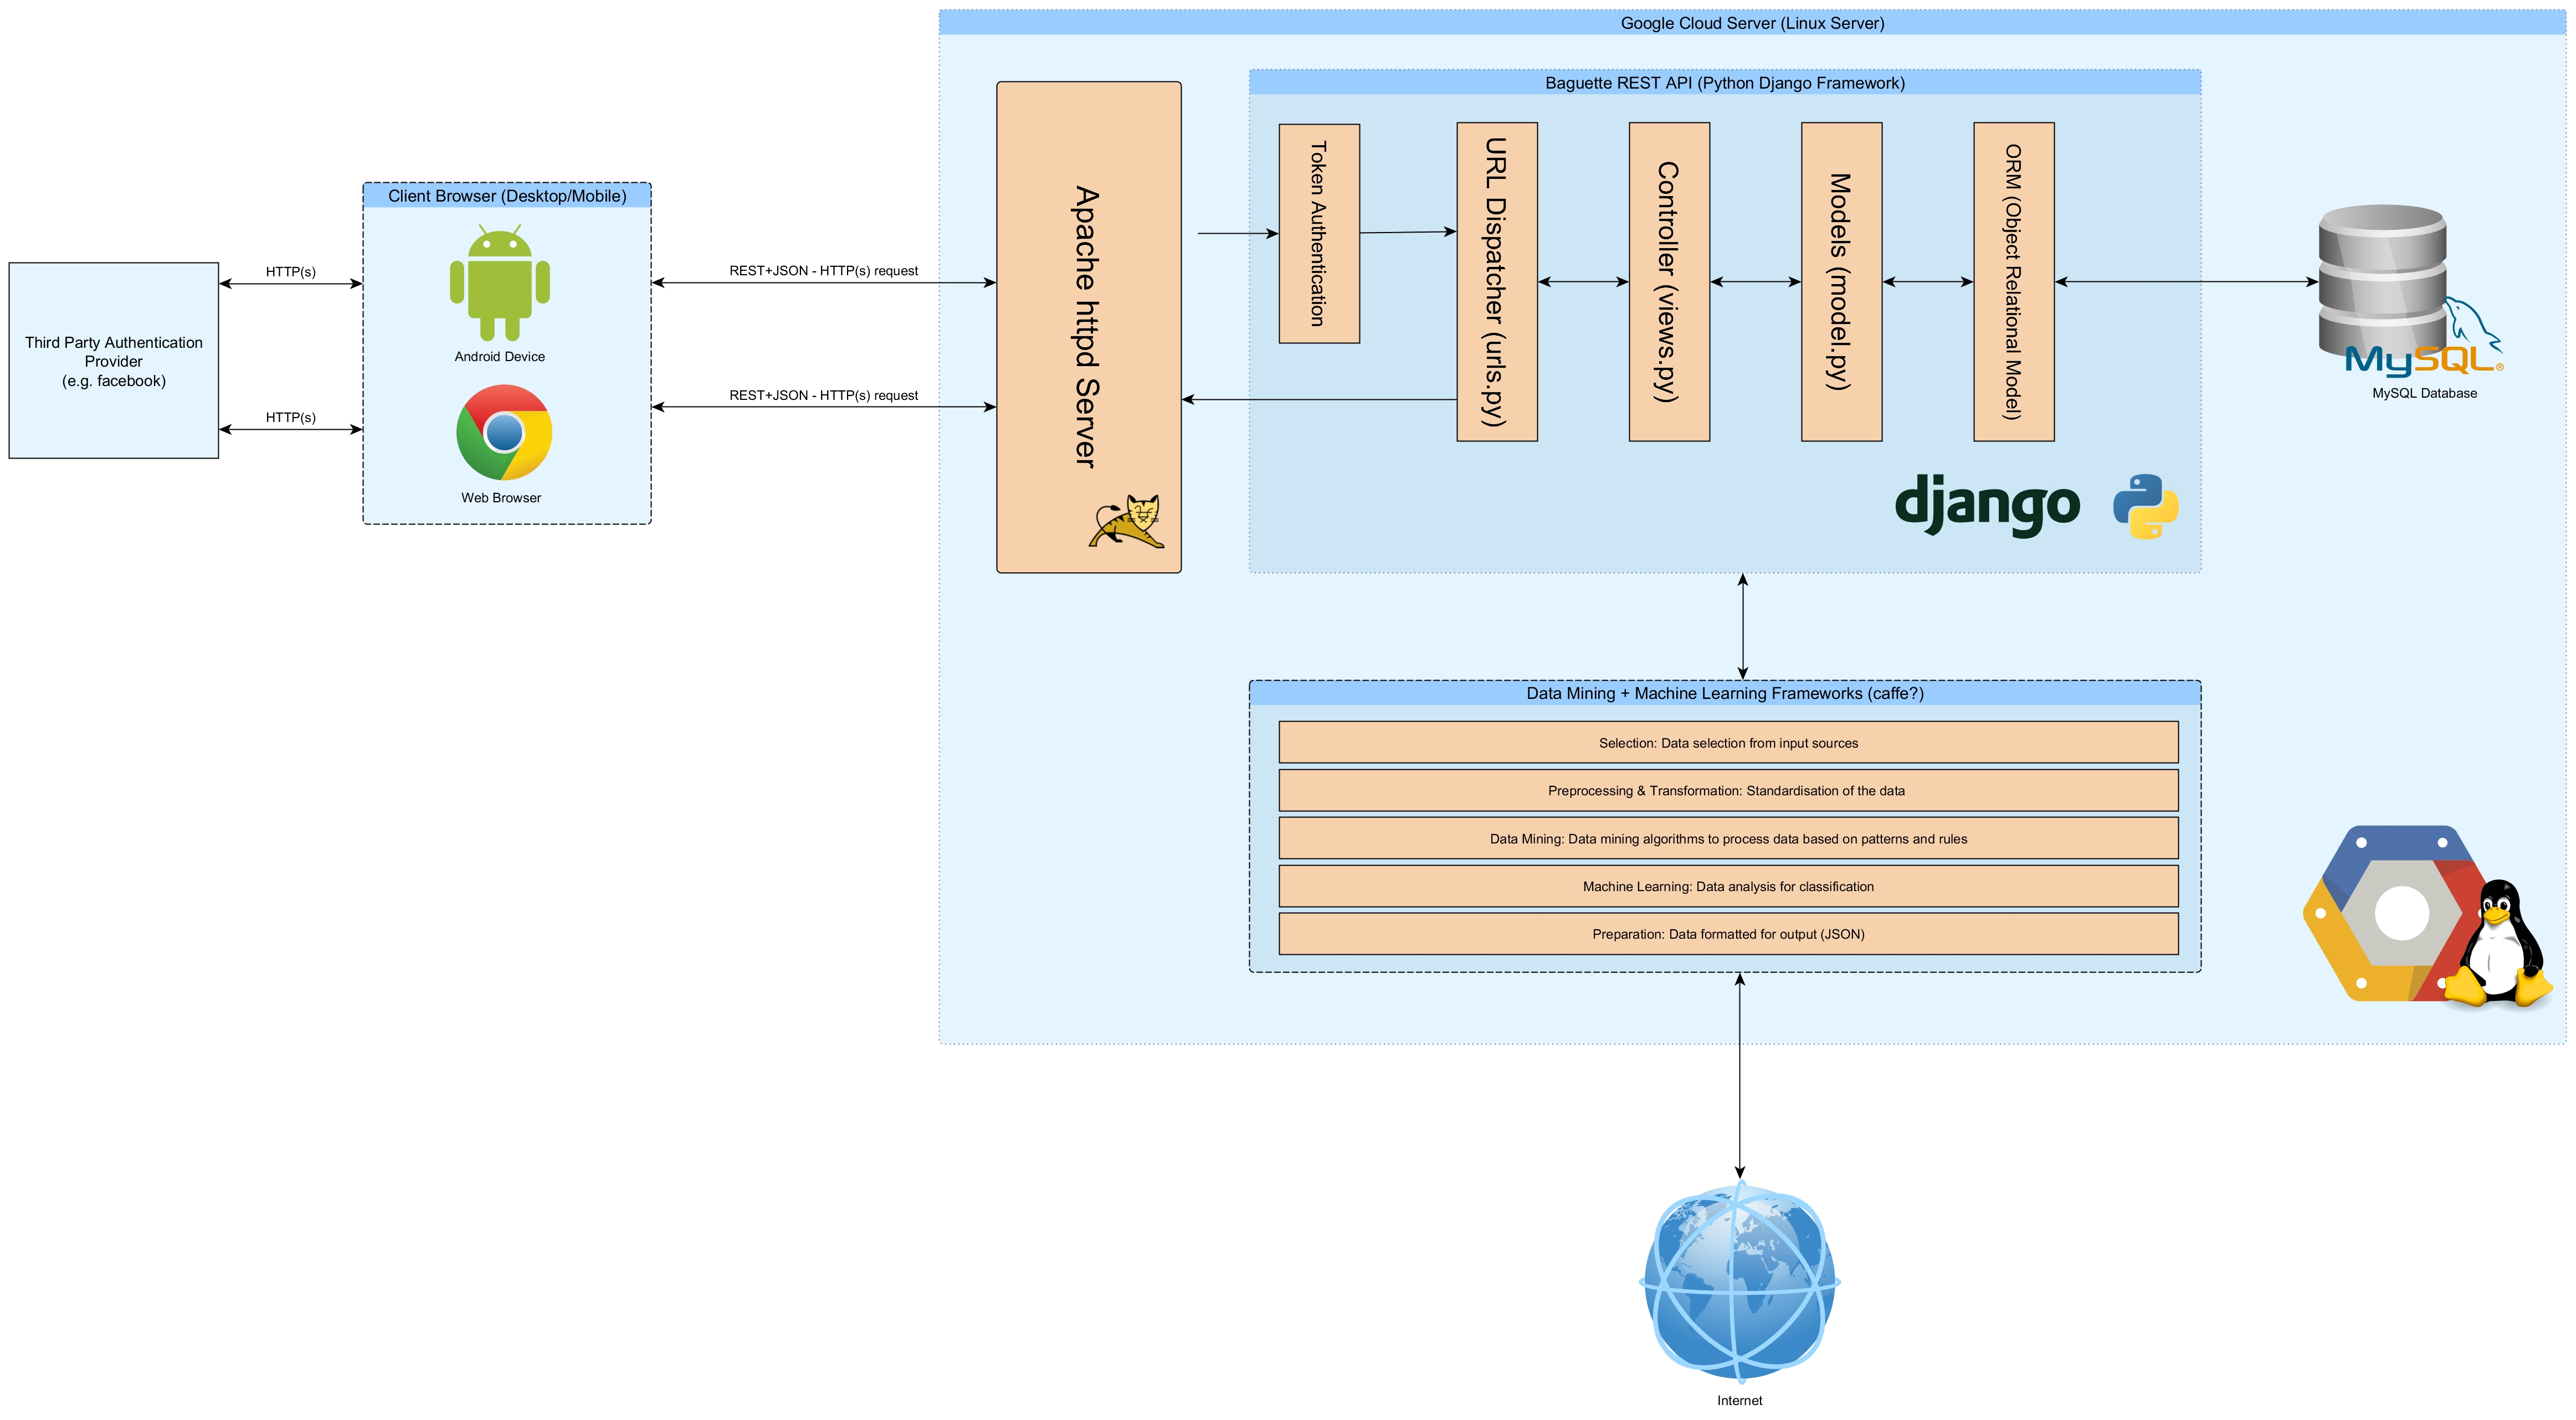
\includegraphics[width=180mm]{inc/architecture_diagram.jpg}
    \caption{System Architecture Diagram}
    \label{fig:architecture_diagram}
  \end{minipage}
\end{figure}

\end{landscape}
